\documentclass[11pt,a4paper]{article}
\usepackage[utf8]{inputenc}
\usepackage[T1]{fontenc}
\usepackage[spanish,es-noshorthands]{babel}
\usepackage{amsmath,amssymb,amsthm}
\usepackage{bm}
\usepackage{geometry}
\geometry{margin=2.5cm}
\usepackage{graphicx}
\graphicspath{{../figuras/}}
\usepackage{float}
\usepackage{xcolor}
\usepackage{hyperref}
\hypersetup{colorlinks=true,linkcolor=blue!50!black,citecolor=blue!50!black,urlcolor=blue!50!black}
\usepackage{enumitem}
\usepackage{booktabs}
\newtheorem{definition}{Definición}
\newtheorem{remark}{Observación}
\newcommand{\R}{\mathbb{R}}
\newcommand{\x}{\mathbf{x}}
\newcommand{\thetavec}{\bm{\theta}}
\newcommand{\transp}{^{\top}}
\title{\textbf{M5 --- Aprendizaje científico: Neural ODE y PINN}\\[2pt]
\large Redes que aprenden física: dinámica vs.\ solución, y por qué funcionan}
\author{Proyecto Wilson--Cowan --- Iniciación a la I+D ITBA}
\date{\today}

\begin{document}
\maketitle
\tableofcontents
\bigskip

\begin{abstract}
Este documento (núcleo del paquete) explica las dos arquitecturas de \emph{Scientific Machine Learning} (SciML) que usamos para identificar los 10 parámetros de Wilson--Cowan (WC): la \textbf{Neural ODE}, que aprende la \emph{dinámica} $\dot\x=f_\theta(\x)$ e integra para obtener la trayectoria, y la \textbf{PINN}, que aprende directamente la \emph{solución} $t\mapsto\x(t)$ penalizando el residuo físico de las ecuaciones. Antes vemos los ingredientes: qué es un MLP y por qué sufre \emph{sesgo espectral}, cómo lo curamos con \emph{Fourier features}, cómo se propaga el gradiente a través del integrador (\emph{adjoint} vs.\ backprop directo), el enfoque \emph{gray-box}/UDE, el \emph{multiple shooting} y la reparametrización \emph{softplus} para positividad. Cerramos con una tabla comparativa y la conexión con el control: la Neural ODE sirve de gemelo digital de la planta, la PINN no. \\
\textbf{Requiere:} M2 (EDOs y sistemas dinámicos), M3 (integración numérica y rigidez), M4 (optimización y descenso por gradiente). \textbf{Conecta con:} B5 (control en lazo cerrado) y P4 (código \texttt{neural\_ode}).
\end{abstract}

% ==========================================================================
\section{El problema y las dos rutas}
\label{sec:problema}
El estado de WC es $\x=[I,E]$ (tasas de disparo inhibitoria y excitatoria) y su dinámica, con offsets de reposo $k_e,k_i$ y sigmoidea $S_a(u)=1/(1+e^{-au})$ (ver M2, B3):
\begin{align}
  \dot I &= \tfrac{1}{\tau_i}\big(-I + S_i(w_{IE}E - w_{II}I + Q(t) - \theta_i) - k_i\big),\label{eq:wcI}\\
  \dot E &= \tfrac{1}{\tau_e}\big(-E + S_e(w_{EE}E - w_{EI}I + P(t) - \theta_e) - k_e\big),\label{eq:wcE}
\end{align}
con $P(t)\!\to\!E$, $Q(t)\!\to\!I$ los estímulos y $\thetavec$ los 10 parámetros a recuperar. La salida observada es $y(t)=E(t)-I(t)$. \textbf{Identificar} es hallar $\thetavec$ a partir de trayectorias medidas con ruido.

Hay dos maneras de meter la física en una red:
\begin{itemize}[nosep]
  \item \textbf{Neural ODE:} aprender la \emph{regla de cambio} $f_\theta:(\x,P,Q)\mapsto\dot\x$ e \emph{integrarla} para reproducir la trayectoria. El estímulo es entrada explícita.
  \item \textbf{PINN:} aprender la \emph{trayectoria} $\x_\theta:t\mapsto\x(t)$ como función del tiempo, exigiendo que satisfaga \eqref{eq:wcI}--\eqref{eq:wcE} vía un término de pérdida. El estímulo queda implícito (una red por trayectoria).
\end{itemize}
Ambas comparten el mismo bloque constructor --- un perceptrón multicapa --- y la misma herramienta que las hace posibles: la \emph{diferenciación automática}. Empezamos por ahí.

% ==========================================================================
\section{Redes neuronales: MLP, activaciones y sesgo espectral}
\label{sec:mlp}

\subsection{El MLP como aproximador de funciones}
Un \emph{perceptrón multicapa} (MLP) es una función parametrizada que compone capas afines seguidas de una no linealidad $\sigma$ \cite{goodfellow2016}. Con entrada $\mathbf{z}_0$ y capas $\ell=1,\dots,L$:
\begin{equation}
  \mathbf{z}_\ell = \sigma\!\big(W_\ell\,\mathbf{z}_{\ell-1} + \mathbf{b}_\ell\big),\qquad
  \mathrm{MLP}(\mathbf{z}_0)=W_{L}\,\mathbf{z}_{L-1}+\mathbf{b}_{L}.
\end{equation}
Los pesos $W_\ell$ y sesgos $\mathbf{b}_\ell$ son los parámetros aprendibles. El \emph{teorema de aproximación universal} garantiza que, con suficientes neuronas, un MLP puede aproximar cualquier función continua en un compacto tan bien como se quiera; en la práctica lo que importa no es la existencia sino qué tan \emph{fácil} es que el descenso por gradiente (ver M4) encuentre esa aproximación.

\paragraph{Funciones de activación.} La no linealidad $\sigma$ es lo que distingue un MLP de una regresión lineal (sin ella, la composición de capas afines colapsa a una sola afín). Las usuales:
\begin{itemize}[nosep]
  \item \textbf{tanh} / \textbf{sigmoidea}: suaves y acotadas, con derivadas de todo orden. \emph{Convenientes para PINN}, porque el residuo físico \eqref{eq:pinn} deriva la red respecto de $t$ por autograd y una activación suave da derivadas limpias.
  \item \textbf{ReLU} ($\max(0,x)$): barata y sin saturación, domina en visión; pero su segunda derivada es nula casi en todos lados, lo que la vuelve pobre cuando se necesitan derivadas de la salida.
  \item \textbf{softplus} ($\log(1+e^x)$): versión suave de ReLU; la reusaremos en la Sección~\ref{sec:softplus} para forzar positividad de parámetros.
\end{itemize}

\subsection{Sesgo espectral y Fourier features}
Un MLP entrenado con descenso por gradiente exhibe un \emph{sesgo espectral} (\emph{spectral bias}): aprende primero las componentes de \textbf{baja frecuencia} de la función objetivo y le cuesta muchísimo capturar las de alta frecuencia \cite{tancik2020}. Intuitivamente, los modos suaves reducen la pérdida más rápido, así que el optimizador los prioriza y las oscilaciones rápidas quedan sin representar.

Esto es un problema directo para nosotros: en el régimen \emph{theta--gamma} objetivo, la salida $y(t)$ tiene ráfagas gamma rápidas moduladas por una envolvente theta lenta. Una PINN que mapea $t\mapsto\x$ con un MLP crudo aplanaría el gamma.

\paragraph{La cura: Fourier features.} En vez de alimentar la red con $t$ directamente, se mapea $t$ a un vector de senos y cosenos con un banco de frecuencias $B=\{b_1,\dots,b_m\}$ \emph{antes} de la primera capa:
\begin{equation}
  \gamma(t)=\big[\sin(2\pi b_1 t),\cos(2\pi b_1 t),\;\dots,\;\sin(2\pi b_m t),\cos(2\pi b_m t)\big].
\end{equation}
Con esta codificación, representar una oscilación de frecuencia $b_k$ ya no exige que el MLP la ``invente'': se la damos servida como coordenada de entrada. Así la red puede aprender los ritmos rápidos del modelo sin necesidad de crecer en tamaño, y el sesgo espectral deja de ser una barrera. La Figura~\ref{fig:sesgo} lo ilustra.

\begin{figure}[H]\centering
  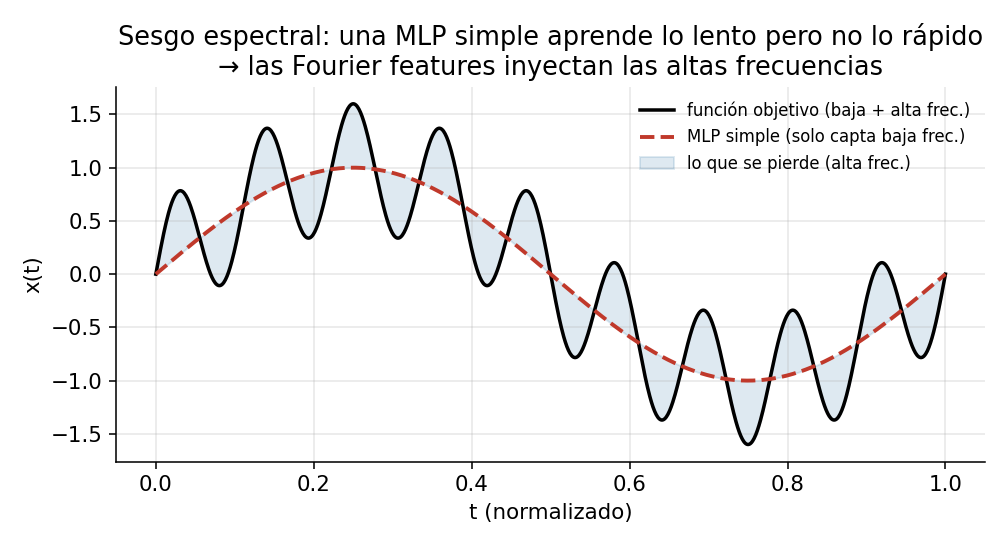
\includegraphics[width=0.75\linewidth]{fig_sesgo_espectral.png}
  \caption{Sesgo espectral: un MLP simple capta la componente de baja frecuencia de la señal pero pierde la de alta frecuencia; el mapeo por \emph{Fourier features} le entrega las oscilaciones rápidas como coordenadas de entrada y permite recuperarlas.}
  \label{fig:sesgo}
\end{figure}

% ==========================================================================
\section{Neural ODE: aprender la dinámica}
\label{sec:node}

\begin{definition}[Neural ODE]
Modelo en el que la \emph{derivada} del estado la da una función parametrizada, y la salida se obtiene \textbf{integrando} esa derivada \cite{chen2018}:
\begin{equation}
  \dot\x = f_\theta(\x,t),\qquad
  \x(t_1)=\x(t_0)+\int_{t_0}^{t_1} f_\theta(\x(t),t)\,dt.
\end{equation}
\end{definition}
La intuición nace de las ResNets: un bloque residual $\mathbf{h}_{n+1}=\mathbf{h}_n+f(\mathbf{h}_n)$ es exactamente \emph{un paso de Euler} de una EDO; al hacer los pasos infinitesimales, la red profunda tiende a un límite continuo, y ese límite es la Neural ODE \cite{chen2018}. En vez de aprender la función entrada$\to$salida, aprende su \emph{tasa de cambio}.

\subsection{Integración y su costo (recordatorio de M3)}
Para evaluar la salida hay que \emph{resolver} la EDO numéricamente. El proyecto usa \textbf{RK4 de paso fijo} (orden 4, 4 evaluaciones de $f$ por paso, diferenciable). El costo se mide en \emph{número de evaluaciones de $f$} (NFE): con RK4, $\mathrm{NFE}=4\times\text{pasos}$. Cuán chico debe ser $\Delta t$ lo fija la \emph{rigidez} del sistema (ver M3); WC es poco rígido y admite pasos grandes, pero con estímulos conmutados (pulsos, escalones optogenéticos) un $\Delta t$ grande degrada la identificación por el error del retenedor de orden cero en cada conmutación.

\subsection{Backprop a través del solver}
Entrenar significa integrar $f_\theta$ y minimizar el error contra la trayectoria medida (\emph{rollout}):
\begin{equation}
  \mathcal{L}(\thetavec)=\big\lVert \mathrm{rollout}(f_\theta,\x_0,P,Q,\Delta t)-\mathbf{y}_{\text{medido}}\big\rVert^2.
\end{equation}
Como el integrador RK4 es una \emph{composición de operaciones diferenciables}, se puede propagar el gradiente $\partial\mathcal{L}/\partial\thetavec$ por \emph{backpropagation a través del solver} (autograd desenrolla todos los pasos). Es simple y exacto, pero guarda en memoria todas las etapas intermedias del rollout.

\paragraph{El método adjoint.} La alternativa que popularizó el paper original \cite{chen2018} evita guardar las activaciones: calcula el gradiente resolviendo \emph{una segunda EDO hacia atrás} en el tiempo (la ecuación \emph{adjunta})
\begin{equation}
  \dot{\mathbf{a}}(t)=-\,\mathbf{a}(t)\transp\,\frac{\partial f_\theta}{\partial \x},
\end{equation}
de modo que todos los gradientes salen de una sola pasada del solver sobre un estado aumentado, con memoria $O(1)$ respecto de la longitud de la trayectoria. Es la técnica de elección para horizontes largos. \textbf{En este proyecto usamos backprop directo}: como entrenamos por trayectorias \emph{cortas} (ver \emph{multiple shooting} abajo), la memoria no es el cuello de botella y el desenrollado directo es más simple y estable.

\subsection{Enfoque gray-box / UDE}
\label{sec:graybox}
En lugar de una red genérica de caja negra ($f_\theta=$ MLP puro), usamos un \emph{backbone} con la \textbf{estructura exacta} de \eqref{eq:wcI}--\eqref{eq:wcE} y parámetros $\thetavec$ aprendibles, más una corrección neuronal \emph{opcional} $g_\phi$ --- es una \emph{Universal Differential Equation} (UDE) \cite{rackauckas2020}:
\begin{equation}
  f_\theta(\x,P,Q)=\underbrace{f_{\mathrm{WC}}(\x,P,Q;\thetavec)}_{\text{física conocida}}
  \;+\;\underbrace{g_\phi(\x,P,Q)}_{\text{corrección (off por defecto)}}.
\end{equation}
Ventajas de este \emph{gray-box}:
\begin{enumerate}[nosep,label=(\roman*)]
  \item \textbf{Parámetros interpretables:} lo que se aprende son los pesos y umbrales de WC, no pesos opacos de una red --- se pueden leer, comparar con la biología y diagnosticar con Fisher+SVD (ver M6).
  \item \textbf{Estructura para el control:} conservar la forma de las ecuaciones permite que el controlador cancele el acoplamiento E--I y prediga la respuesta a $P,Q$ (ver B5).
  \item \textbf{Costo despreciable de red:} con la corrección \emph{apagada} (el defecto), el ``modelo'' son $\sim 10$ escalares. Todo el costo computacional está en la \emph{integración}, no en pasar datos por una red; entrenar es casi tan barato como simular WC.
\end{enumerate}
La corrección $g_\phi$ se activa solo cuando se sospecha que los datos no son exactamente WC (dinámica no modelada): entonces $g_\phi$ absorbe el residuo estructural sin romper la interpretabilidad del backbone.

\subsection{Multiple shooting}
\label{sec:shooting}
Integrar \emph{de un tirón} una trayectoria larga es numéricamente inestable: pequeños errores de parámetro se amplifican a lo largo del rollout y el gradiente ``explota'' (la sensibilidad de la solución final respecto de $\thetavec$ crece de forma casi exponencial en dinámicas oscilatorias). La cura clásica \cite{bock1984} es el \emph{multiple shooting}: se parte la trayectoria en \textbf{ventanas cortas}, cada una \textbf{reiniciada desde el estado observado} en su borde inicial, y solo se integra dentro de la ventana.
\begin{itemize}[nosep]
  \item Cada ventana es un horizonte corto $\Rightarrow$ el gradiente no explota y el problema queda mejor condicionado.
  \item Reduce la memoria del backprop (y justifica usar backprop directo en vez de adjoint).
  \item Precio: un pequeño sesgo por los reinicios, ya que el estado observado tiene ruido. En la práctica es un intercambio muy favorable: estabilidad de entrenamiento a cambio de una perturbación acotada.
\end{itemize}

% ==========================================================================
\section{PINN: aprender la solución}
\label{sec:pinn}

\begin{definition}[PINN --- \emph{Physics-Informed Neural Network}]
Una red que aproxima la \emph{solución} $\x_\theta(t)\approx[I(t),E(t)]$ como función del tiempo, entrenada con dos términos \cite{raissi2019}:
\begin{equation}
  \mathcal{L}=\underbrace{\lambda_d\,\lVert \x_\theta(t_i)-\mathbf{y}_i\rVert^2}_{\text{datos}}
  \;+\;\underbrace{\lambda_p\,\big\lVert \dot\x_\theta(t)-f_{\mathrm{WC}}(\x_\theta(t);\thetavec)\big\rVert^2}_{\text{residuo físico}}.
  \label{eq:pinn}
\end{equation}
\end{definition}
El primer término ajusta la red a los datos observados; el segundo la obliga a \emph{satisfacer las ecuaciones de WC} en un conjunto de puntos de colocación. Los parámetros $\thetavec$ se optimizan \textbf{junto} con los pesos de la red: la física no es solo un chequeo, es lo que hace identificable a $\thetavec$.

\paragraph{La derivada por autograd (clave para el ruido).} El $\dot\x_\theta(t)$ del residuo no se calcula por diferencias finitas sobre los datos, sino por \emph{diferenciación automática} de la red respecto de su entrada $t$. Esto es central: estimar $\dot\x$ por diferencias finitas sobre señales ruidosas \emph{amplifica} el ruido (dividir diferencias chicas), mientras que autograd deriva la función suave $\x_\theta$, que la red ya suavizó al ajustar los datos. Es la ventaja frente a los métodos de \emph{derivative matching} clásicos (tipo SINDy), que sí necesitan derivar los datos y sirven de baseline de comparación.

\paragraph{Fourier features, otra vez.} Como la PINN mapea $t\mapsto\x$ con un MLP, sufre el sesgo espectral de la Sección~\ref{sec:mlp}. Por eso también aquí se anteponen \emph{Fourier features} $\gamma(t)$ a la red, para captar los ritmos rápidos del régimen theta--gamma.

\paragraph{Lecciones de entrenamiento (medidas en el proyecto).} El balance $\lambda_d,\lambda_p$ es delicado: con el peso físico demasiado alto la red cae en un \emph{mínimo degenerado} (satisface la física con parámetros errados); con el de datos demasiado alto los parámetros no se mueven. Entrenar los dos términos en \emph{etapas separadas} rompe el acoplamiento (gradiente $\approx 0$). La receta que funciona es \textbf{entrenamiento conjunto} (datos + física a la vez), \textbf{multi-trayectoria} (un mismo $\thetavec$ compartido por varias trayectorias) y $\lambda_d$ alto, con Fourier features.

% ==========================================================================
\section{Reparametrización softplus para positividad}
\label{sec:softplus}
Varios parámetros de WC deben ser \emph{estrictamente positivos}: las constantes de tiempo $\tau_e,\tau_i$ y las ganancias sigmoideas $a_e,a_i$. En vez de imponer una restricción dura al optimizador (que introduce fronteras donde el gradiente se comporta mal), se aprende una variable \emph{libre} $\rho\in\R$ y se define el parámetro vía \emph{softplus}:
\begin{equation}
  \theta=\mathrm{softplus}(\rho)=\log(1+e^{\rho})>0.
\end{equation}
Es suave, monótona e invertible, así que el gradiente fluye sin barreras y el parámetro nunca cruza el cero. El optimizador de M4 trabaja en $\rho$ (sin restricciones) y la física ve siempre un $\theta$ válido.

\paragraph{Offsets $k_e,k_i$ derivados, no aprendidos.} Los offsets de reposo de \eqref{eq:wcI}--\eqref{eq:wcE} \textbf{no se aprenden libres}. Se \emph{derivan} de los otros parámetros para que el reposo $E=I=0$ sea equilibrio sin estímulo:
\begin{equation}
  k_e=\frac{1}{1+e^{a_e\theta_e}},\qquad
  k_i=\frac{1}{1+e^{a_i\theta_i}}.
\end{equation}
Al restarlos, con $P=Q=0$ el término no lineal cancela exactamente el estado nulo y $\dot E=\dot I=0$. Dejarlos libres agregaría una \emph{degeneración} extra (dos parámetros que compensan lo mismo), justo lo que queremos evitar en un problema de identificación ya mal condicionado (ver M6).

% ==========================================================================
\section{PINN vs.\ Neural ODE: cuándo cada una}
\label{sec:comparacion}
Las dos arquitecturas resuelven el mismo problema por caminos opuestos. La Figura~\ref{fig:pvn} resume la comparación del proyecto; la Tabla~\ref{tab:comp} la sistematiza.

\begin{figure}[H]\centering
  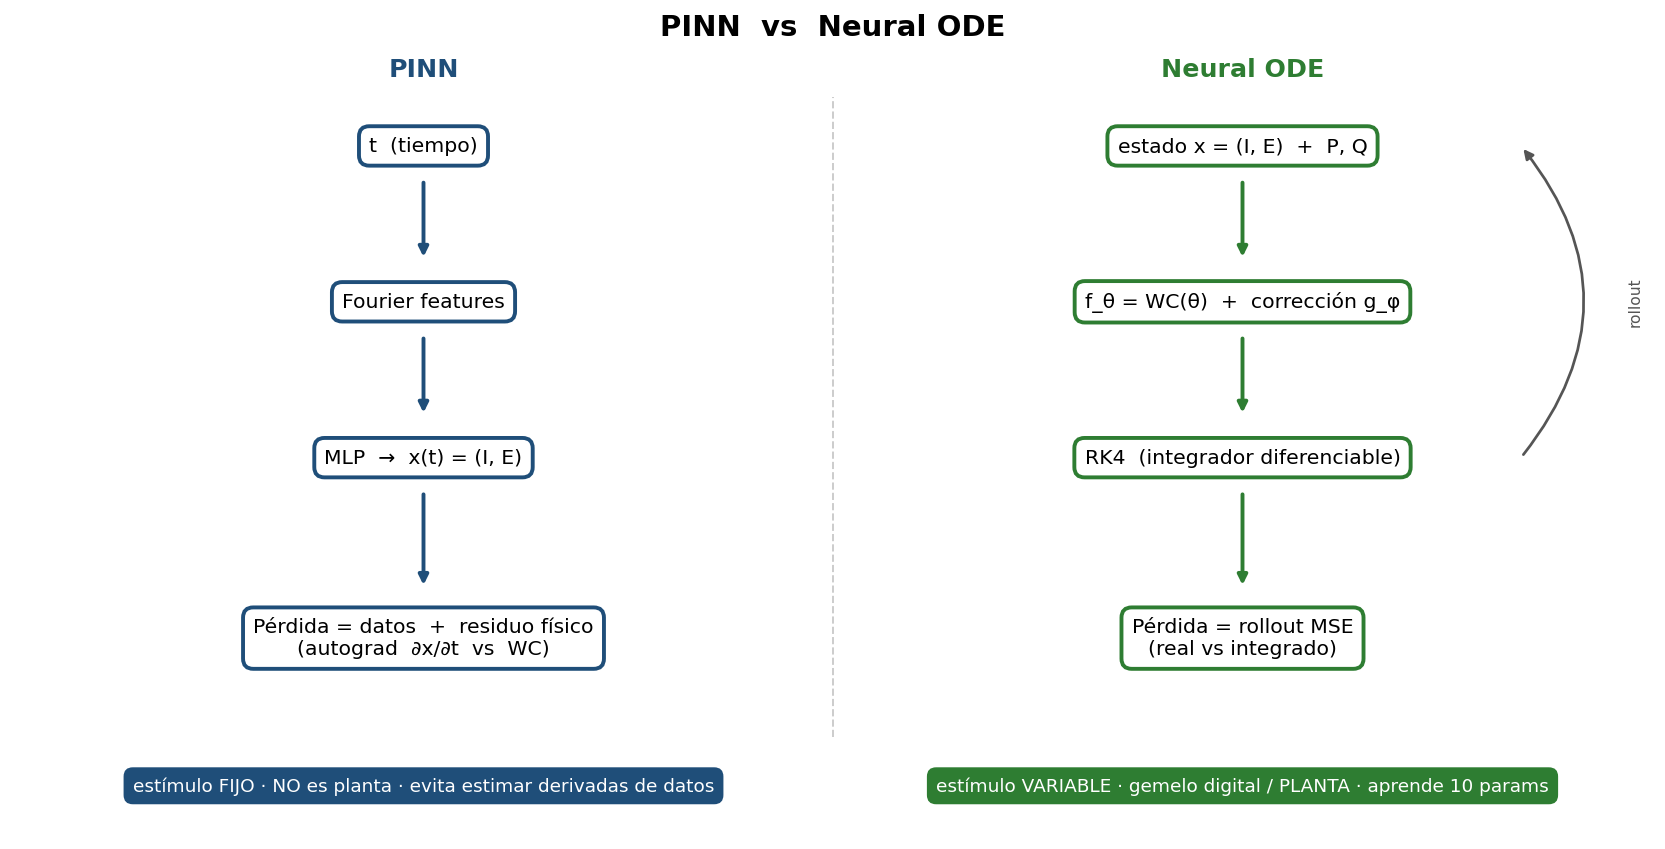
\includegraphics[width=0.75\linewidth]{pinn_vs_node.png}
  \caption{Comparación PINN vs.\ Neural ODE en la identificación de Wilson--Cowan (figura del proyecto): qué aprende cada una y su desempeño relativo.}
  \label{fig:pvn}
\end{figure}

\begin{table}[H]\centering
\begin{tabular}{@{}lll@{}}
\toprule
 & \textbf{PINN} & \textbf{Neural ODE} \\
\midrule
Qué aprende        & solución $t\mapsto\x$              & dinámica $(\x,P,Q)\mapsto\dot\x$ \\
Derivadas          & autograd en $t$                   & integración numérica (rollout) \\
Estímulo           & fijo (una red por trayectoria)    & variable / en línea (entrada explícita) \\
Uso en control     & no directo                        & sí (gemelo digital / planta) \\
Costo dominante    & tamaño de red                     & integración (NFE) \\
Robustez a ruido   & suaviza nativamente               & vía suavizado + ventanas (shooting) \\
Denoising          & implícito en la red               & requiere multiple shooting \\
\bottomrule
\end{tabular}
\caption{Comparación operativa PINN vs.\ Neural ODE.}
\label{tab:comp}
\end{table}

\paragraph{Resultados medidos.} En corridas limpias ambas identifican los 4 pesos con error sub-porcentual; en el proyecto la Neural ODE llegó a identificar los \emph{10} parámetros desde un arranque ignorante con error máximo $\sim 1.1\%$. La Figura~\ref{fig:chirp} muestra un ajuste sobre una trayectoria de test tipo \emph{chirp} (frecuencia creciente), donde la identificación limpia reproduce fielmente la dinámica.

\begin{figure}[H]\centering
  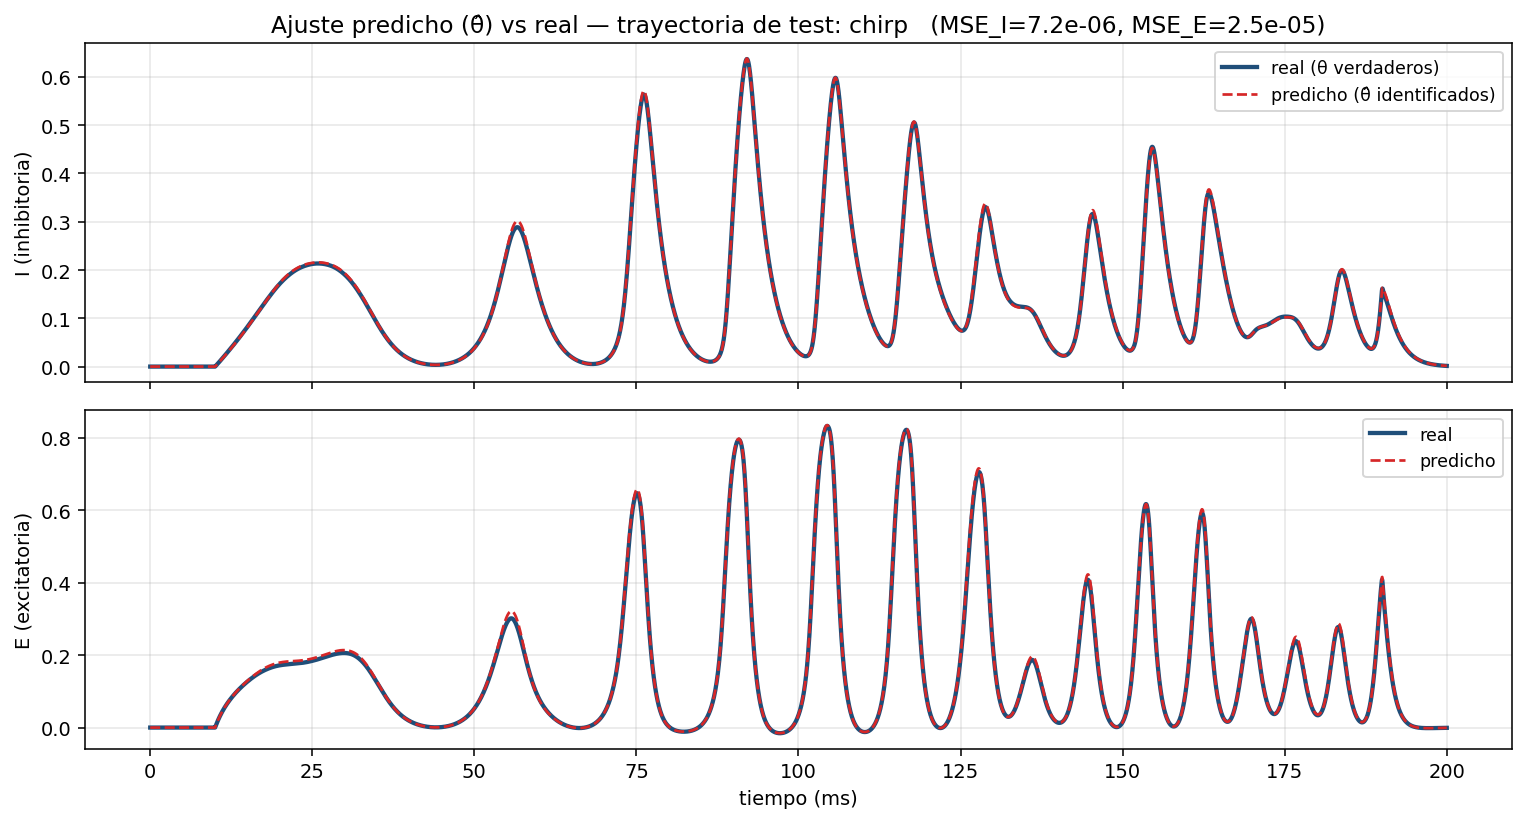
\includegraphics[width=0.75\linewidth]{fit_chirp_test.png}
  \caption{Ajuste del modelo identificado sobre una trayectoria de test tipo \emph{chirp} (figura del proyecto): la dinámica aprendida generaliza a un estímulo de frecuencia variable no visto en entrenamiento.}
  \label{fig:chirp}
\end{figure}

\paragraph{La diferencia que decide el proyecto.} La PINN mapea $t\mapsto\x$ para un estímulo \emph{fijo}: no se le puede cambiar la entrada sobre la marcha, así que \textbf{no sirve como planta de un lazo de control}. La Neural ODE mapea $(\x,P,Q)\mapsto\dot\x$ con el estímulo como entrada explícita: \emph{un solo modelo} responde a cualquier $P,Q$, por lo que puede integrarse en un lazo donde los estímulos se generan en línea. Por eso la Neural ODE es el \textbf{gemelo digital} de la planta y la que alimenta al controlador IMC (ver B5); la PINN es una excelente herramienta de \emph{identificación} pero no de \emph{control}.

\paragraph{Regla práctica.} Usar \textbf{PINN} cuando el objetivo es identificar $\thetavec$ a partir de una o pocas trayectorias con ruido y no hace falta simular estímulos nuevos (denoising nativo, sin solver). Usar \textbf{Neural ODE} cuando se necesita un modelo \emph{ejecutable} que responda a estímulos arbitrarios --- identificación orientada al control, generación de trayectorias, gemelo digital.

% ==========================================================================
\section{Conexión con la identificabilidad y el control}
\label{sec:conexion}
Ni la PINN ni la Neural ODE eliminan por sí solas las \emph{degeneraciones} del problema (p.\,ej.\ que $w_{II}$ viva en una dirección casi plana del paisaje de pérdida). De eso se ocupa el análisis de Fisher$+$SVD (ver M6): decide \emph{qué} parámetros son recuperables, \emph{cuáles} fijar o regularizar y \emph{qué} estímulo inyectar (diseño óptimo de experimentos, OED). Estas redes son el \emph{motor de ajuste}; el diagnóstico de identificabilidad es el \emph{mapa}.

El objetivo final es cerrar el lazo: los parámetros identificados por la Neural ODE alimentan un controlador IMC en lazo cerrado (ver B5), y la acción integral del controlador vuelve el seguimiento robusto al error residual de identificación --- de ahí que la fragilidad de $w_{II}$ no se propague al control. La implementación de todo esto (backbone gray-box, rollout RK4, softplus, multiple shooting) vive en el código \texttt{neural\_ode} (ver P4).

% ==========================================================================
\begin{thebibliography}{99}
\bibitem{chen2018} R.~T.~Q.~Chen, Y.~Rubanova, J.~Bettencourt y D.~Duvenaud, ``Neural Ordinary Differential Equations'', \emph{NeurIPS}, 2018.
\bibitem{raissi2019} M.~Raissi, P.~Perdikaris y G.~E.~Karniadakis, ``Physics-informed neural networks: A deep learning framework for solving forward and inverse problems involving nonlinear PDEs'', \emph{J.\ Comput.\ Phys.}, 378:686--707, 2019.
\bibitem{rackauckas2020} C.~Rackauckas \emph{et al.}, ``Universal Differential Equations for Scientific Machine Learning'', preprint arXiv:2001.04385, 2020.
\bibitem{bock1984} H.~G.~Bock y K.~J.~Plitt, ``A multiple shooting algorithm for direct solution of optimal control problems'', \emph{IFAC Proceedings}, 17(2):1603--1608, 1984.
\bibitem{tancik2020} M.~Tancik \emph{et al.}, ``Fourier features let networks learn high frequency functions in low dimensional domains'', \emph{NeurIPS}, 2020.
\bibitem{goodfellow2016} I.~Goodfellow, Y.~Bengio y A.~Courville, \emph{Deep Learning}, MIT Press, 2016.
\end{thebibliography}

\end{document}
